Our analysis of the SLOSH data's extremal dependence requires some background.
    \makenote{introduce the review section.  avoid naked sections.}

\subsection{Extreme Value Theory\label{ref:evt}}
\begin{comment}
    \begin{itemize}
        \item Formal introduction of extreme analysis
        \begin{itemize}
            \item Separation of angular and radial components
        \end{itemize}
    \end{itemize}
\end{comment}
\makenote{first paragraph basically copy-pasted from ndpg.  Rephrase more?}
Extreme value theory uses the limited information available in a sample to
    characterize the tails of a distribution.  In the univariate case, asymptotic
    results provide a unique parametric limiting family for the maximum observation
    in a sample.  For data with such a limiting distribution, a common approach
    is to consider observations in excess of a high threshold, and model the
    excesses over that threshold under a generalized Pareto framework.  This
    approach is known as \emph{peaks over threshold} (PoT).  In the multivariate 
    case, the theory for PoT is well established (see, for example, 
    \cite{dehaan2006}), and it indicates the existence of a limiting distribution
    with no parametric representation.  This can pose a challenge for inference,
    but we are not without options.

The multivariate PoT model considered in this paper has been developed 
    in~\cite{trubey:pg}, based on a definition of the limiting distribution proposed
    proposed in~\cite{rootzen2018}.  
    Let $\bm{W} = (W_1,\ldots,W_d)$ be a $d$--dimensional random vector with 
    cumulative distribution $F$.  Assuming there exists a sequence of vectors
    $\bm{a}_n$, $\bm{b}_n$, and a $d$--variate distribution $G$ such that 
    $\lim\limits_{n\to\infty}F^n(\bm{a}_n\bm{w} + \bm{b}_n) = G(\bm{w})$, then
    $G$ is a $d$--variate generalized extreme value distribution.  Then,
    \begin{equation}
        \label{eqn:threshold}
        \lim\limits_{n\to\infty}\text{Pr}
            \left[\bm{a}_n^{-1}(\bm{W} - \bm{b}_n) 
                \leq \bm{w}\mid \bm{W}\not\leq \bm{b}_n\right]
        = \frac{\log G(\bm{w}\wedge \bm{0}) - \log G(\bm{w})}{\log G(\bm{0})}
        = H(\bm{w})
    \end{equation}
    where $H$ is the multivariate Pareto distribution.  \cite{rootzen2018}
    provides a number of stochastic representations of $H$, and in particular,
    Remark~1 justifies the representation given in \cite{ferreira2014} where,
    in the limit, we factorize $\bm{W} = R\bm{V}$ with $R$ and $\bm{V}$ independent.
    \makenote{I'm not very fond of this transition.  We standardize $\bm{W}$ to 
    $\bm{Z}$, then factorize $\bm{Z} = R\bm{V}$.  Separability holds true in both
    cases (i think), but in the former. $\bm{V}$ is still dependent on the marginal 
    distributional parameters.  Standardization allows those to be ignored.  
    We should mention standardization before factorization.}
    $R = \lVert \bm{W}\rVert_{\infty}$ is distributed as a standard Pareto random
    variable, and $\bm{V} = \bm{W} / \lVert \bm{W}\rVert_{\infty}$ is a random
    vector existing within $\mathbb{S}_{\infty}^{d-1}$, the positive orthant of
    the unit sphere under the $\mathcal{L}_{\infty}$ norm.  $R$ and $\bm{V}$
    respectively comprise the \emph{radial} and \emph{angular} components of $H$.
    As $R$ and $\bm{V}$ are independent,  the distribution of $\bm{V}$ is 
    effectively the dependence structure of $\bm{W}$.

Let the threshold $b_{qs} = \hat{F}_{s}^{-1}(1 - q)$, where $\hat{F}$ is
    the empirical cumulative distribution function for the $s$th component.
    Marginally, values exceeding the threshold $b_{qs}$ are assumed to follow
    a univariate generalized Pareto distribution, and are used to estimate the
    corresponding marginal scale and shape parameters $a_{s}$ and $\xi_{s}$
    respectively.  Setting $\bm{b}$ and having inferred $\bm{a}$, and $\bm{\xi}$, 
    we transform $\bm{w}\mid \bm{w}\not\leq \bm{b}$ to a standard multivariate 
    Pareto form via the transformation
    \begin{equation}
        \label{eqn:standardization}
        z_{is} = \left(1 + \xi_{s}\frac{w_{is} 
            - b_{s}}{a_{s}}\right)_{+}^{1 / \xi_{s}}
    \end{equation}
    where $(\cdot)_+$ indicates the positive parts function.  Let 
    $r_i = \lVert \bm{z}_i\rVert$, and $\bm{v}_i = \bm{z}_i / r_i$.  Due to 
    thresholding, $i$ ranges from 1 to $m\leq n$, and $r_i > 1$.  Recall that
    $R\in (1, \infty)$ will, by design, follow a standard Pareto distribution,
    the inferential task left to us is describing the distribution of the
    angular component $\bm{V}\in\mathbb{S}_{\infty}^{d-1}$.  

\subsection{Projected Gamma\label{ref:pg}}
\begin{comment}
    \begin{itemize}
        \item Introduction of Projected gamma distribution
        \begin{itemize}
            \item Projected Gamma as the kernel density of a BNP mixture
        \end{itemize}
    \end{itemize}
\end{comment}
A suitable distribution for $\bm{V}$ can be approximated by projecting a 
    distribution in $\mathbb{R}_+^d$ onto $\mathbb{S}_{p}^{d-1}$.  
    Recall the $\mathcal{L}_p$ norm 
    $\lVert \bm{x}\rVert_p = \left(\sum_{s = 1}^dx^p\right)^{1/p}$.  Then
    for $\bm{x}\in\mathbb{R}_+^d$, we define the transformation
    \begin{equation}
        \label{eqn:projection}
        T_p(\bm{x}) = \left(\lVert \bm{x}\rVert_p, 
            \frac{x_1}{\lVert \bm{x}\rVert_p},\ldots, 
                \frac{x_{d-1}}{\lVert \bm{x}\rVert_p}\right)
                =: (r,\bm{y})
    \end{equation}
    where $y = (y_1,\ldots,y_{d-1}) \in \mathbb{S}_{p}^{d-1}$, $r > 0$, and 
    $y_d = (1 - \sum_{s = 1}^{d-1}y_{s}^p)^{\frac{1}{p}}$.
    By transforming $\bm{x}$ to $(r,\bm{y})$ and integrating out $r$, we
    succeed in establishing a distribution for $\bm{y}$ on 
    $\mathbb{S}_{\infty}^{d-1}$
    The Jacobian of the transformation in Equation~\eqref{eqn:projection} is
    $r^{d-1}[Y_d + \sum_{s = 1}^{d-1}y_{s}^py_d^{1-p}]$.
    This Jacobian is well suited to a product of gammas density, where 
    $f(\bm{x}\mid\bm{\alpha},\bm{\beta}) = 
        \prod_{s = 1}^d\mathcal{G}(x_{s}\mid\alpha_{s},\beta_{s})$.
    Transforming $\bm{x}$ as described, $r$ can be integrated out in closed
    form, leaving the \emph{projected gamma} density for arbitrary $p > 0$.
    \[
        f(\bm{y}\mid\bm{\alpha},\bm{\beta}) = \prod_{s = 1}^d\left[
            \frac{\beta_{s}^{\alpha_{s}}}{\Gamma(\alpha_{s})}
            y_{s}^{\alpha_{s} - 1}\right]
            \left[y_d + \sum_{s = 1}^{d-1}y_{s}^py_d^{1-p}\right]
            \frac{\Gamma(\sum_{s = 1}^d \alpha_{s})}{\left(
                \sum_{s = 1}^d\beta_{s}y_{s}
                \right)^{\sum_{s = 1}^d \alpha_{s}}
            }
    \]
    Of course, at $p=\infty$, the transformation is not differentiable, so a 
    direct projection onto $\mathbb{S}_{\infty}^{d-1}$ is not possible. We
    instead desire a high but finite $p$.
    Here we balance two issues: as $p\to\infty$, the space $\mathbb{S}_{p}^{d-1}$ 
    will approach asymptotically towards $\mathbb{S}_{\infty}^{d-1}$.
    Unfortunately, also as $p\to\infty$, the stability of the Jacobian of the
    transformation becomes increasingly dependent on the value, or choice, of 
    $y_d$.  If $y_d\to 0$, then the Jacobian diverges, and the distribution 
    becomes numerically unstable. We select $p = 10$ to balance these concerns.

To more faithfully capture the structure of the data, we use the projected gamma density 
    as a kernel density of an Bayesian non-parametric mixture model, based on 
    the Pitman-Yor process introduced in~\cite{perman1992}.  A Pitman-Yor process
    is a fully atomic measure specified by two parameters and a centering
    distribution.  Under a stick-breaking representation as described 
    in~\cite{ishwaran2001}, 
    \[
        \text{Pr}(\bm{\alpha}\mid\ldots) 
            = \sum_{j = 1}^Jp_j\delta_{\bm{\alpha}_j};\;\;\;
            \sum_{j=1}^Jp_j = 1;\;\;\;
            p_j := \chi_j\prod_{k = 1}^{j-1}(1 - \chi_k)
    \]
    where $\delta_{\bm{\alpha}_j}$ indicates a point mass at $\bm{\alpha}_j$ and
    $\bm{\alpha}_j$ are sampled independently from the centering distribution $G_0$.
    Under the Pitman-Yor process, $\chi_j \sim \text{Beta}(1 - d, \eta + jd)$
    where $d \in [0, 1)$ denotes the \emph{discount} parameter and $\eta > -d$
    denotes the \emph{concentration} parameter.

For the rest of this paper, let $i$ denote indexing over storm simulations (observations), 
    specifically those which survived the thresholding necessitated by the assumption of 
    Equation~\eqref{eqn:threshold}.  Let $s \in \lbrace 1, \ldots, S\rbrace$ denote indexing 
    over locations t which the storm surge is simulated.  That is, $y_{is}$ is the maximum simulated
    storm surge at location $s$ during storm $i$, after projection onto $\mathbb{S}_p^{d-1}$.
    Let $j\in \lbrace 1,\ldots,J\rbrace$ denote indexing over \emph{clusters}, the aforementioned
    mixture components up to truncation point $J$.  Then, the model can be specified as
    \begin{equation}
        \begin{aligned}
            \bm{y}_i \mid \bm{\alpha}_i &\sim
                \mathcal{PG}_p\left(\bm{Y}\mid\bm{\alpha}_i,\bm{1}\right)\\
            \bm{\alpha}_i &\sim G\\
            G &\sim \mathcal{PY}\left(\eta, \zeta, G_0\right)        
        \end{aligned}
        ~\hspace{1cm}
        \begin{aligned}
            G_0 &= {\textstyle\prod}_{s = 1}^{S}\mathcal{G}(\alpha_{s}\mid \xi_{s},\tau_{s})\\
            \xi_{s} &\sim \mathcal{G}(\xi\mid a, b)\\
            \tau_{s} &\sim \mathcal{G}(\tau\mid c, d)
        \end{aligned} 
    \end{equation}
    where $\eta$ and $\zeta$ are respectively the concentration and discount parameters
    of the Pitman--Yor process.  Fitting this model for a moderate number of sites can be 
    accomplished via Markov-chain Monte Carlo methods.  Using the collapsed Gibbs sampler,
    We introduce a latent cluster assignment variable $\delta_i$ for each storm $i$ which 
    indicates which cluster storm $i$ belongs to.  Then the posterior distribution of

\subsection{SLOSH}
\begin{comment}
    \begin{itemize}
        \item More in-depth discussion of dataset
        \begin{itemize}
            \item Break dataset down into 3 levels of analysis; t90, all--but--road--features, airports.
            \item Descriptive statistics thereof
            \item Pitfalls in analysis?
        \end{itemize}
    \end{itemize}
\end{comment}

The projected gamma based model is not an inherently spatial model.  
    \makenote{change reasoning such that we are interested in \emph{specific} locations
    rather than change from grid to specific locations being due to computational
    complexity.}
    As such, rather than holding the entire grid in memory, it makes sense to consider 
    data pertaining only to landmarks of interest.    If one is performing 
    contingency planning in preparation for the storm season, it would be 
    helpful to know the probability of such services being rendered inoperable 
    simultaneously, precisely when they are needed most.  If one is seeking 
    sites for a new service provider, it would be helpful understand the 
    likelihood of a proposed location being rendered inoperable in the same 
    manner.  For these reasons, and considering the computational complexity of 
    a 23 million dimensional model, rather than consider the entire grid of data 
    pertaining to any particular storm, we subset the data to grid cells in the 
    vicinity of such locations of interest.  These locations are gathered from 
    the 2023 US Census Bureau's \emph{TIGER} database \needcite and specifically 
    the point and landmark file.  If a grid cell falls within 70 meters of a location,
    then the grid cell is identified with the location.  If multiple grid cells
    are within 70 meters, then the nearer one is identified with the location.
    Additionally, we select locations, or grid cells, that have experienced at
    at least some inundation in some $q$ proportion of storm simulations.  That is,
    such that $b_{qs} > 0$, for all $s$ of interest.  This restriction arises
    as a consequence of fitting the parameters for the marginal generalized Paretos:
    if the threshold for excesses $b$ is not set above $0$, the likelihood can diverge, 
    and MLE estimation of the parameters suffers. Here we experience another
    tradeoff, the implications of which are explored in 
    Figure~\ref{fig:thresholdselection}.  Setting a higher threshold allows more 
    sites to be included in the analysis, but in turn reduces the number of storm 
    simulations which exceed the threshold in at least one dimension.  This in turn 
    reduces the amount of information available by which we can estimate the 
    dependence structure.

\begin{figure}[ht]
    \centering
    \caption{Trade-offs in threshold specification:
    \makenote{remake with better labels}
    (Left) Proportion of sites with threshold $b_{qs} > 0$ versus $(1 - q)$; 
    (Right) Proportion of storms $\bm{W}_i \not< \bm{b}_q$ versus $(1-q)$.
    \label{fig:thresholdselection}}
    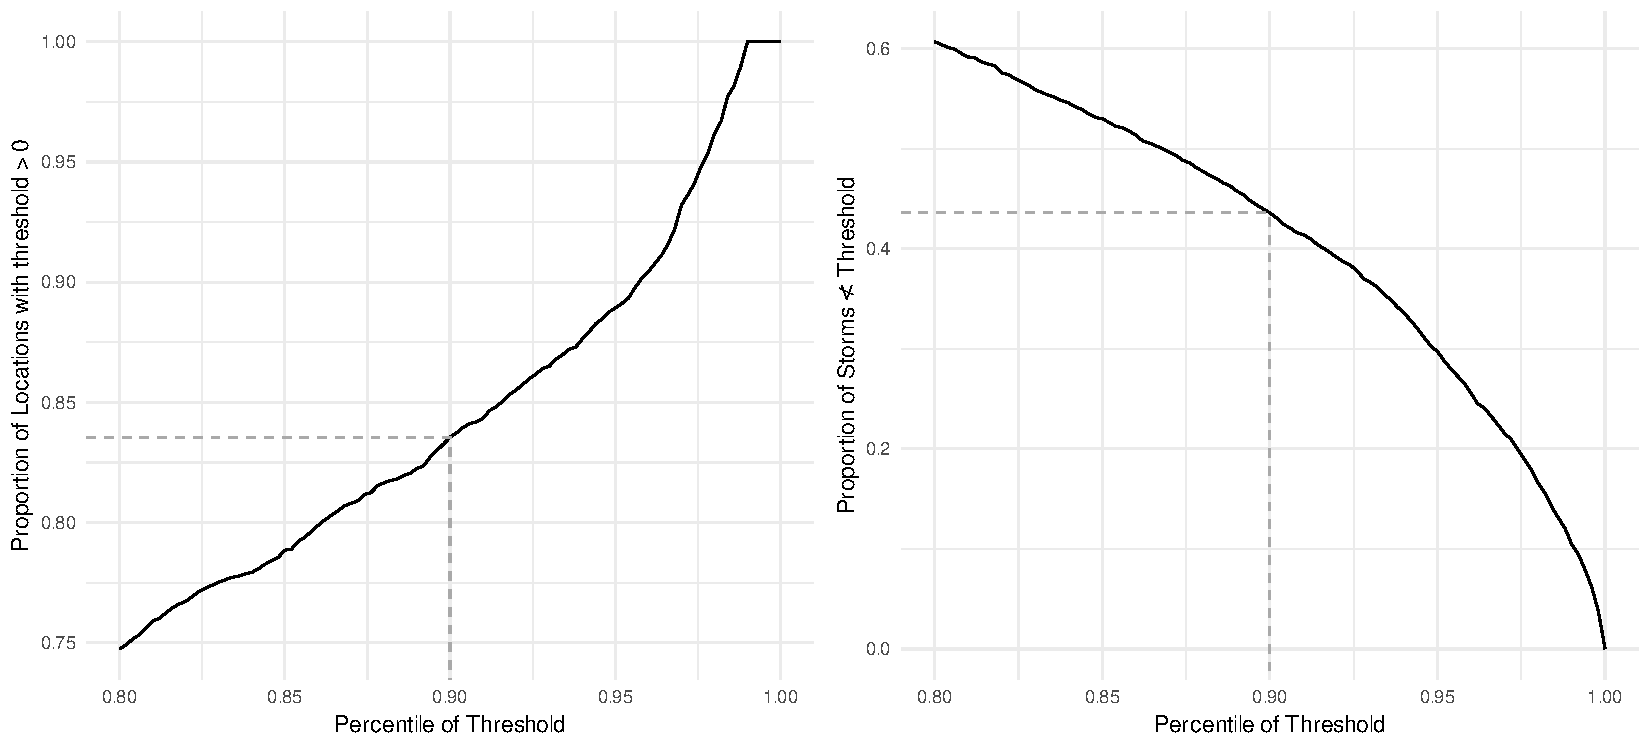
\includegraphics[width=0.9\linewidth]{plots/explore_threshold}
\end{figure}

\begin{table}
    \centering
    \caption{Table of Dataset Slices\label{tab:datasets}}    
\end{table}

At this point, we split the analysis into three parts.  First, we look at locations
    pertaining to critical services, which if rendered unable to operate could
    drastically increase the negative effects, or loss of life, due to the storm.
    This means isolating locations in the dataset specific to critical services, or
    other locations of interest.  This is the \emph{critical services} dataset.  We
    set the threshold in this dataset at the marginal 95\% quantile.
    \makenote{mention feature class codes used}
    Second, we look at the overall shape of the storm inundation field in order to
    use the clustering action of the Pitman-Yor process model to find emergent clusters
    of storm characteristics.  For this purpose, we are interested in a large sample
    size, with a large number of locations.  We select the threshold at the 90\% quantile, 
    and select all identified locations with at least some inundation at that quantile.
    The resulting number of locations---and number of storms exceeding the threshold---for 
    each of the analysis datasets is delineated in Table~\ref{tab:datasets}.
    \makenote{airports dataset?}

\begin{figure}[b]
    \centering 
    \caption{Histogram of storm characteristics for storm simulations 
        which surived thresholding.\label{fig:thetahistogram}}
    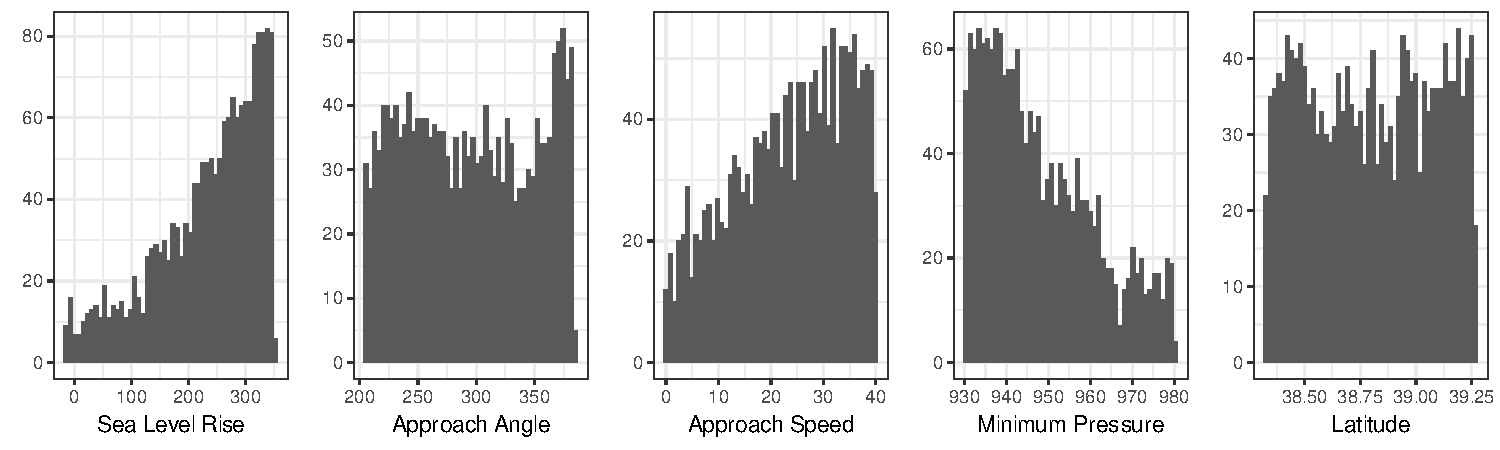
\includegraphics[width=0.9\linewidth]{plots/threshold_histogram}
\end{figure}

Figure~\ref{fig:thetahistogram} shows the marginal histograms of storm parameters, for 
    storms which survived thresholding in the 90\% threshold dataset.  Storm parameters in 
    the originating dataset were sampled via Latin hypercube, so would appear marginally
    uniform.  The difference between marginal uniform, and the observed densities provides
    some indication of what characteristics are necessary for a storm to exceed the threshold.
    In the first case, for sea level rise, it is readily apparent that a higher sea level will
    make it easier for a storm to inundate larger swaths of land, or inundate locations to a
    greater degree.  So we expect to see, and do see, a higher probability of a storm exceeding
    the threshold, for a higher sea level rise.  Similarly, a lower minimum pressure in the storm's
    eye corresponds to a more intense storm.  We expect to see, and do see, a higher percentage of
    exceeding the threshold, for a lower minimum pressure.  The relationship to approach speed is 
    interesting in that it's almost linear.  Perhaps, the mechanism there lies in that a higher
    approach speed indicates more power behind the storm.  The spike in approach angle past 360
    degrees is interesting as well. 360 degrees indicates due North, thus approach angles 
    beyond 360 degrees indicate the storm is heading slightly northeast. As these approaches are
    on the eastern seaboard, this indicates a shallower approach angle relative to the
    land---perhaps offering a given storm more time to inundate larger swaths of land.

% EOF 